\subsection{Premesse}

Per progettare un circuito che legga il segnale elettrico del nostro battito cardiaco a livello della cute, dobbiamo considerare che:
\begin{itemize} [noitemsep]
	\item Sulla superficie del corpo il segnale ECG è normalmente di circa \SI{1}{mV} (al massimo raggiunge i \SI{4}{mV}) ed ha una frequenza di circa \SI{1.25}{\Hz}.
	\item Gli elettrodi a nostra disposizione, che realizzano il collegamento tra la strumentazione e il corpo, creano un potenziale di circa \SI{700}{\mV}, quindi di circa \num{3} ordini di grandezza maggiore del segnale cardiaco.
	\item Il segnale da misurare è piccolo, quindi dobbiamo porre particolare attenzione alle fonti di rumore elettromagnetico dati da effetti capacitivi e/o induttivi. Inoltre dobbiamo evitare che i cavi e il paziente si muovano durante la misurazione.
	\item È necessario che il paziente sia isolato dal lato di elaborazione del segnale, alimentato dall'alimentatore da banco, per evitare problemi di giri di massa.
\end{itemize}

Tenendo conto di questi aspetti, nei paragrafi successivi analizzeremo gli aspetti legati all'abbattimento dei rumori e all'amplificazione del segnale in ingresso.

\subsection{Abbattimento dei rumori}

Questo primo stadio in entrata (operazionale U1 in Figura \ref{cir8:compensation}) è necessario per avere un'alta impedenza in ingresso (e dunque un valore maggiormente fedele alla reale ddp del corpo), per eliminare i segnali di modo comune generati dagli elettrodi e per richiedere una prima amplificazione (dato il basso valore di tensione in entrata).

In testa ed in coda a questo stadio sono però presenti delle capacità che creano due filtri: rispettivamente un passa basso ed un passa alto.

\paragraph{Passa Basso} Posto in testa ad U1, e composto dalle capacità $C_c$ e $C_d$, è necessario per abbattere eventuali rumori ambientali causati dalle radio-frequenze. Date le capacità in Figura \ref{cir8:compensation}, il datasheet dell'operazionale ci fornisce le seguenti frequenze di taglio di modo differenziale
\begin{equation*}
	\frac{1}{2 \pi R ( C_d + C_c ) } = \SI{194}{\Hz}
\end{equation*}
e di modo comune
\begin{equation*}
	\frac{1}{2 \pi R C_c} = \SI{4}{\kHz}
\end{equation*}

\paragraph{Passa Alto} La frequenza di taglio è pari a circa \SI{3}{\Hz} (applicando la solita formula della frequenza di taglio di un passa alto). Essendo posto all'uscita dell'operazionale (capacità $C_1$ in Figura \ref{cir8:compensation}, elimina eventuali segnali continui in output. Inoltre, è necessario che questa tensione abbia impedenze adattate, ovvero dovrà essere vista come infinita in entrata al prossimo blocco: per far ciò poniamo un ulteriore operazionale (un OP07, U2 in Figura \ref{cir8:compensation}).

\subsection{Active gards}
Polarizzo la calza del cavo coassiale che connette l’elettrodo all’amplificatore ad un
potenziale pari alla tensione di modo comune.
In tal modo riduco l’effetto delle capacità parassite, e aumento la reiezione di modo
comune.
\begin{itemize}
\item il cavo che porta il segnale “vede” una differenza di potenziale molto bassa. Limito le
perdite nell’isolante
\item entrambi i cavi “vedono” lo stesso potenziale, indipendentemente dalla loro posizione sul
banco)
\end{itemize}

\subsection{Amplificatore di isolamento}
Isola galvanicamente i 2 lati del circuito: quello collegato al paziente ed alimentato a batteria e quello di uscita ed elaborazione del segnale alimentato dall’alimentatore da
banco.
\begin{itemize}
	\item Isola fino a 1500 volt -Alimentazione da+/-4,5V a +/-18V.
	\item Possiede 2 alimentazioni separate e quindi anche due riferimenti di massa separati.
	\item Non richiede componenti esterni (tranne le capacità di disaccoppiamento)
\end{itemize}


\begin{figure}[tpc]
\centering
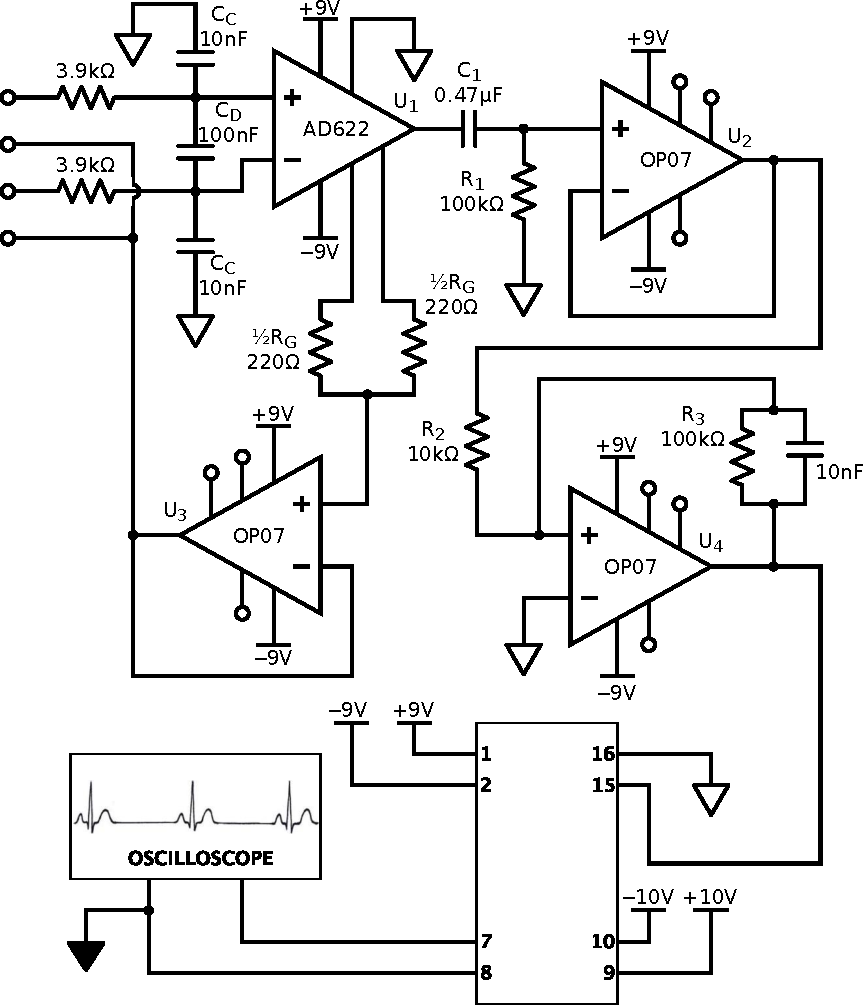
\includegraphics[width=.7\textwidth]{../E07/latex/circuito.pdf}
\caption{Schema del circuito da noi utilizzato per acquisire l'elettrocardiogramma.}
\label{cir8:compensation}
\end{figure}

Questa prima amplificazione è data dalla (\ref{eq5:guadagno_AD622}), e si attesta a $\approx 116$.